\setcounter{chapter}{2}
\chapter{Theorem-like environments}

\begin{frame}
\frametitle{Some results (I)}
\begin{theorem}[Pythagoras]
For a right triangle with sides $a, b$ and hypotenuse $c$, we have
\[
a^2 + b^2 = c^2.
\]
\end{theorem}

An illustration of the Pythagorean theorem is shown in Figure \ref{fig:pythagorean}.

\begin{figure}
\centering
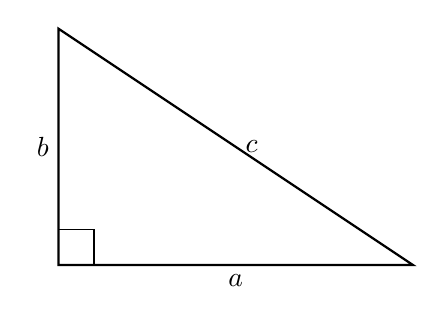
\begin{tikzpicture}[scale=1.5]
    % Triangle coordinates
    \coordinate (A) at (0,0);
    \coordinate (B) at (3,0);
    \coordinate (C) at (0,2);

    % Draw triangle
    \draw[thick] (A) -- (B) -- (C) -- cycle;

    % Right angle marker at A
    \draw (0.3,0) -- (0.3,0.3) -- (0,0.3);

    % Label sides
    \draw[below] (A) -- (B) node[midway, below] {$a$};
    \draw[left] (A) -- (C) node[midway, left] {$b$};
    \draw[above right] (B) -- (C) node[midway, right] {$c$};
\end{tikzpicture}
\caption{A right triangle illustrating the Pythagorean theorem: $a^2 + b^2 = c^2$.}
\label{fig:pythagorean}
\end{figure}

\end{frame}

\begin{frame}
\frametitle{Some results (II)}
\begin{definition}[Prime Number]
A prime number is an integer greater than 1 that has no positive divisors other than 1 and itself.
\end{definition}

\begin{example}[Small Primes]
The first few prime numbers are $2, 3, 5, 7, 11$.
\end{example}

\begin{lemma}[Divisibility Property]
If a prime $p$ divides the product $ab$, then $p$ divides $a$ or $p$ divides $b$.
\label{lemma:divisibility_property}
\end{lemma}

\begin{corollary}
If a prime $p$ divides the product $abc$, then $p$ divides $a$, or $p$ divides $b$, or $p$ divides $c$.
\label{corollary:divisibility_property}
\end{corollary}

\begin{exercise}
Prove Corollary \ref{corollary:divisibility_property} using Lemma \ref{lemma:divisibility_property}.
\end{exercise}

\end{frame}

\begin{frame}
\frametitle{Some results (III)}
\begin{proposition}[Infinitude of Primes]
There are infinitely many prime numbers.
\end{proposition}

\begin{proof}
Assume there are finitely many primes \(p_1,\dots,p_n\). Consider
\[
P = p_1 p_2 \cdots p_n + 1.
\]
Then \(P\) is either prime itself or divisible by a prime not in the list. In either case, there exists a prime not in \(\{p_1,\dots,p_n\}\), contradicting finiteness. Hence, there are infinitely many primes.
\end{proof}

\begin{remark}[Euclid]
The proof of the infinitude of primes, originally due to Euclid, is one of the oldest and most elegant arguments in mathematics.
\end{remark}

\begin{example}[Non-Prime Numbers]
The integers $4, 6, 8, 9, 10$ are not prime, since each can be expressed as a product of smaller integers.
\label{ex:non_prime}
\end{example}
\end{frame}

\begin{frame}
\frametitle{Some results (IV)}
\begin{pyexercise}{Go to Jupyter and run Exercise~\ref{ex:non_prime_py}.}
\begin{mdcell}
As stated in Example `\ref{ex:non_prime}`{=tex}, we verify that $6$ is not prime by checking that $6 = 2 \cdot 3$.
\end{mdcell}
\begin{pycell}
assert 6 == 2 * 3
\end{pycell}
\mode<all>
\label{ex:non_prime_py}
\end{pyexercise}

\begin{remark}
In Exercise~\ref{ex:non_prime_py} we could have also used a larger number, say $8$, $9$ or $10$. See Exercise~\ref{ex:non_prime_py_2}.
\end{remark}

\begin{pyexercise}[Variant of Exercise~\ref{ex:non_prime_py}]{Go to Jupyter and run Exercise~\ref{ex:non_prime_py_2}.}
\begin{mdcell}
As stated in Example `\ref{ex:non_prime}`{=tex}, we verify that $10$ is not prime by checking that $10 = 2 \cdot 5$.
\end{mdcell}
\begin{pycell}
assert 10 == 2 * 5
\end{pycell}
\mode<all>
\label{ex:non_prime_py_2}
\end{pyexercise}
\end{frame}
